\documentclass[modern]{aastex61}

% All the packages
%\usepackage[letterpaper]{geometry}
\usepackage{fontspec}
\usepackage{microtype}
\usepackage{url}
\usepackage{amsmath}
\usepackage{mathtools}
\usepackage{esint}
\usepackage{amssymb}
\usepackage{natbib}
\usepackage{multirow}
\usepackage{graphicx}
\usepackage{scalerel}
\usepackage{calc}
\usepackage{etoolbox}
\usepackage{marginnote}
\usepackage{nicefrac}
\usepackage{tabstackengine}
\usepackage{diagbox}
\usepackage[makeroom]{cancel}
\usepackage{mathdots}
\usepackage{bbm}
\usepackage{booktabs}
\usepackage{xspace}
\usepackage{upgreek}
\usepackage[T1]{fontenc} % https://tex.stackexchange.com/a/166791
\usepackage{textcomp}
\usepackage{ifxetex}
\ifxetex
\usepackage{fontspec}
\defaultfontfeatures{Extension = .otf}
\fi
\usepackage{fontawesome}
\usepackage{listings}
\usepackage{mathtools}
\stackMath

% Page breaks in long equations
%\allowdisplaybreaks

% Bibliography stuff
\bibliographystyle{aasjournal}

% Shorthand for this paper
\newcommand{\starry}{\textsf{starry}\xspace}
\newcommand{\batman}{\textsf{batman}\xspace}
\newcommand{\planetplanet}{\textsf{planetplanet}\xspace}
\newcommand{\Python}{\textsf{Python}\xspace}
\newcommand{\cpp}{\textsf{C}++\xspace}
\newcommand{\Mathematica}{\textsf{Mathematica}\xspace}

% editing
\newcommand{\todo}[1]{{\color{red}\textbf{TODO:} #1}}


% References to text content
\newcommand{\documentname}{\textsl{article}}
\newcommand{\figureref}[1]{\ref{fig:#1}}
\newcommand{\Figure}[1]{Figure~\figureref{#1}}
\newcommand{\figurelabel}[1]{\label{fig:#1}}
\renewcommand{\eqref}[1]{\ref{eq:#1}}
\newcommand{\Eq}[1]{Equation~(\eqref{#1})}
\newcommand{\eq}[1]{\Eq{#1}}
\newcommand{\eqalt}[1]{Equation~\eqref{#1}}
\newcommand{\eqlabel}[1]{\label{eq:#1}}

% Add code, proof, and animation hyperlinks
\definecolor{linkcolor}{rgb}{0.1216,0.4667,0.7059}
\newcommand{\codeicon}{{\color{linkcolor}\faFileCodeO}}
\newcommand{\prooficon}{{\color{linkcolor}\faPencilSquareO}}
\newcommand{\animicon}{{\color{linkcolor}\faPlayCircle}}
\input{gitlinks}

\newtagform{eqtag}[]{(}{)}
\newcommand{\currentlabel}{None}

% Define a proof environment
\newenvironment{proof}[1]{%
\ifstrempty{#1}{%
\renewtagform{eqtag}[]{\raisebox{-0.1em}{{\color{red}\faPencilSquareO}}\,(}{)}%
}{%
\renewtagform{eqtag}[]{\prooflink{#1}\,(}{)}%
}%
\usetagform{eqtag}%
\renewcommand{\currentlabel}{#1}
\align%
}{%
\endalign%
\renewtagform{eqtag}[]{(}{)}%
\usetagform{eqtag}%
\message{<<<\currentlabel: \theequation>>>}%
}

% Define a proof environment
\newenvironment{proof*}[1]{%
\ifstrempty{#1}{%
\renewtagform{eqtag}[]{\raisebox{-0.1em}{{\color{red}\faPencilSquareO}}\,(}{)}%
}{%
\renewtagform{eqtag}[]{\prooflink{#1}\,(}{)}%
}%
\usetagform{eqtag}%
\renewcommand{\currentlabel}{#1}
\equation%
}{%
\endequation%
\renewtagform{eqtag}[]{(}{)}%
\usetagform{eqtag}%
\message{<<<\currentlabel: \theequation>>>}
}

% Math stuff
%\newcommand{\ii}{\ensuremath{\mathbf{i}}}
\newcommand{\T}{\ensuremath{\mathrm{T}}}
\newcommand{\dd}{\ensuremath{ \mathrm{d}}}
\newcommand{\unit}[1]{{\ensuremath{\mathrm{#1}}}}
\newcommand{\bvec}[1]{{\ensuremath{\mathbf{#1}}}}
\newcommand{\avec}[1]{{\ensuremath{\vec{\mathbf{#1}}}}}
\newcommand{\x}{\ensuremath{\mbox{$x$}}}
\newcommand{\y}{\ensuremath{\mbox{$y$}}}
\newcommand{\z}{\ensuremath{\mbox{$z$}}}
\newcommand{\xhat}{\ensuremath{\mathbf{\hat{x}}}}
\newcommand{\yhat}{\ensuremath{\mathbf{\hat{y}}}}
\newcommand{\zhat}{\ensuremath{\mathbf{\hat{z}}}}
\DeclareMathAlphabet\mathbfcal{OMS}{cmsy}{b}{n}
\DeclareMathOperator{\Tr}{Tr}
\DeclarePairedDelimiter\ceil{\lceil}{\rceil}
\DeclarePairedDelimiter\floor{\lfloor}{\rfloor}
\definecolor{dim}{rgb}{0.8,0.8,0.8}
\newcolumntype{L}[1]{>{\raggedright\let\newline\\\arraybackslash\hspace{0pt}}m{#1}}
\setcounter{MaxMatrixCols}{20}
\newcommand{\sinphi}{\ensuremath{\mbox{$u$}}}
\newcommand{\sinlambda}{\ensuremath{\mbox{$v$}}}
\newcommand{\bigdot}{\scaleto{\cdot}{6pt}}

% Bases
\newcommand{\ubasis}{\ensuremath{\tilde{\mathbf{u}}}}
\newcommand{\ubasisn}{\ensuremath{\tilde{\mathbf{u}}_n}}
\newcommand{\pbasis}{\ensuremath{\tilde{\mathfrak{p}}}}
\newcommand{\pbasisn}{\ensuremath{\tilde{\mathfrak{p}}_n}}
\newcommand{\gbasis}{\ensuremath{\tilde{\mathfrak{g}}}}
\newcommand{\gbasisn}{\ensuremath{\tilde{\mathfrak{g}}_n}}

% Code examples
\usepackage{listings}
\definecolor{codegreen}{rgb}{0,0.6,0}
\definecolor{codegray}{rgb}{0.5,0.5,0.5}
\definecolor{codepurple}{rgb}{0.58,0,0.82}
\definecolor{backcolour}{rgb}{0.95,0.95,0.95}
\lstdefinestyle{mystyle}{
    backgroundcolor=\color{backcolour},
    commentstyle=\color{codegreen},
    keywordstyle=\color{magenta},
    numberstyle=\tiny\color{codegray},
    stringstyle=\color{codepurple},
    basicstyle=\small\ttfamily,
    breakatwhitespace=false,
    breaklines=true,
    captionpos=b,
    keepspaces=true,
    numbers=left,
    numbersep=5pt,
    showspaces=false,
    showstringspaces=false,
    showtabs=false,
    tabsize=2,
    aboveskip=1em,
    belowskip=1em,
    keywords=[2]{map},
    keywordstyle=[2]{\color{black!80!black}},
}
\lstset{style=mystyle}

% Inverse diagonal dots
\makeatletter
\def\Ddots{\mathinner{\mkern1mu\raise\p@
\vbox{\kern7\p@\hbox{.}}\mkern2mu
\raise4\p@\hbox{.}\mkern2mu\raise7\p@\hbox{.}\mkern1mu}}
\makeatother

% Typography obsessions
\setlength{\parindent}{3.0ex}
\renewcommand\quad{\hskip\fontdimen3\font}

\usepackage{graphicx}

\begin{document}%\raggedbottom\sloppy\sloppypar\frenchspacing

\setlength{\abovedisplayskip}{1.5em}
\setlength{\belowdisplayskip}{1.5em}

\title{%
    Analytical Transit Light Curves for Limb-Darkened Stars
}

\author[0000-0002-0296-3826]{Rodrigo Luger}
\affil{Department~of~Astronomy, University~of~Washington, Seattle, WA}
\author{Eric Agol}
\affil{Department~of~Astronomy, University~of~Washington, Seattle, WA}

\keywords{methods: analytical --- techniques: photometric}

\begin{abstract}
    We derive analytical, closed form solutions for the light curve
    of a planet transiting a star with a limb darkening profile of
    arbitrary order. We provide updated expressions for the linear
    and quadratically limb darkened cases that are numerically stable
    over the entire domain. 
\end{abstract}

% ==============================================================================
% ------------------------------------------------------------------------------
% ------------------------------------------------------------------------------
%
\section{Introduction}
\label{sec:intro}
% ------------------------------------------------------------------------------
% ------------------------------------------------------------------------------
% ==============================================================================

Currently I just copy-pasted some relevant stuff from the \starry paper.
This week I'll organize this into sections and get an outline going.\todo{}

\cite{Gimenez2006} derived transit light curves for a limb-darkening
function
\begin{equation}
I(\mu) = I(1) \left[\sum_{n=1}^N u_n (1-\mu^n) \right],
\end{equation}
where $\mu = \cos{\theta} =\sqrt{1-r^2}$, where $\theta$ is the polar angle measured from the 
sub-observer point), and $u_n$ is a limb-darkening coefficient.  \cite{Gimenez2006}
found an infinite series for computing the limb-darkened light curve for each $u_n$
term.  Here we present closed-form expressions for these terms which can be
easily computed with recursion relations.

\cite{Pal2008} derived the partial derivatives of the quadratic limb-darkening model 
with respect to $b$ and $r$.


% ==============================================================================
% ------------------------------------------------------------------------------
% ------------------------------------------------------------------------------
%
\section{Reparametrization}
\label{sec:reparam}
% ------------------------------------------------------------------------------
% ------------------------------------------------------------------------------
% ==============================================================================

From \citet{MandelAgol2002}, the total flux visible during the occultation of a
body whose surface map is given by $I(x, y) = \sqrt{1 - \x^2 -\y^2}$ may be computed
as
%
\begin{align}
    \label{eq:s2}
    s_2 = \frac{2\pi}{3} \left(1 - \frac{3\Lambda}{2} - \Theta(r - b) \right)
\end{align}
%
where $\Theta(\bigdot)$ is the Heaviside step function and
%
\begingroup\makeatletter\def\f@size{10}\check@mathfonts
\def\maketag@@@#1{\hbox{\m@th\large\normalfont#1}}%
\begin{align}
    \label{eq:biglam}
    \Lambda &=
    \begin{dcases}
          % I don't think we need this: the k^2>1 term is stable as b --> 0!
          %-\frac{2}{3}\left(1 - r^2\right)^\frac{3}{2}
          %& \qquad b = 0
          %
          %\\[1.5em]
          %
          \frac{1}{9 \pi \sqrt{b r}} \Bigg[
                \frac{(r + b)^2 - 1}{r + b}
                \Big(
                    -2r \,
                    \big(
                        2 (r + b)^2 + (r + b)(r - b) - 3
                    \big)
                    K(k^2)
                    &\\ \phantom{XXXX}
                    + 3 (b - r) \, \Pi\big(k^2 (b + r)^2, \, k^2\big)
                \Big)
                - 4 b r (4 - 7 r^2 - b^2) E(k^2)
          \Bigg]
          %
          & \qquad k^2 < 1
          %
          \\[1.5em]
          %
          \frac{2}{9 \pi} \Bigg[
                \big(1 - (r + b)^2\big)
                \Bigg(
                    \sqrt{1 - (b - r)^2} \,
                    K\left(\frac{1}{k^2}\right)
                    + 3 \left(\frac{b-r}{(b+r)\sqrt{1 - (b - r)^2}}\right)
                    &\\ \phantom{XX}
                    \times \Pi\left(\frac{1}{k^2(b+r)^2}, \, \frac{1}{k^2}\right)
                \Bigg)
                - \sqrt{1 - (b - r)^2}
                (4 - 7 r^2 - b^2)
                E\left(\frac{1}{k^2}\right)
          \Bigg]
          %
          & \qquad k^2 \ge 1
    \end{dcases}
\end{align}
\endgroup
%
with
%
\begin{align}
    \label{eq:k2}
    k^2 &= \frac{1 - r^2 - b^2 + 2 b r}{4 b r}
    \quad.
\end{align}

%
In the expressions above, $K(\bigdot)$, $E(\bigdot)$, and $\Pi(\bigdot, \bigdot)$
are the complete elliptic integrals of the first, second kind, and third kind,
respectively, defined as
%
\begin{align}
    \label{eq:elliptic}
    K(k^2) &\equiv \int_0^{\frac{\pi}{2}} \frac{\dd \varphi}{\sqrt{1 - k^2 \sin^2 \varphi}}
    \nonumber \\[0.5em]
    E(k^2) &\equiv \int_0^{\frac{\pi}{2}} \sqrt{1 - k^2 \sin^2 \varphi} \, \dd \varphi
    \nonumber \\[0.5em]
    \Pi(n, k^2) &\equiv \int_0^{\frac{\pi}{2}} \frac{\dd \varphi}{(1 - n \sin^2 \varphi)\sqrt{1 - k^2 \sin^2 \varphi}}
    \quad.
\end{align}
We have transformed the expressions from \citet{MandelAgol2002} using equation
17.7.17 from \citet{Abramowitz1970} which yields equations that are better
behaved in the vicinity of $b=r$.  However, these elliptic integrals are still
subject to numerical instability as $r \rightarrow 1-b$ and $r >> 1$. Through
trial and error, we have found that these instabilities can be removed by combining 
elliptic integrals into a general complete elliptic integral defined as
\begin{equation}
{\rm cel}(m,k_c,p,a,b) = \int_0^{\pi/2} \frac{a\cos^2{\phi} + b\sin^2{\phi}}{\cos^2{\phi}+p\sin^2{\phi}} \frac{d\phi}{\sqrt{\cos^2{\phi}+k_c^2\sin^2{\phi}}},
\end{equation}
where $k_c = \sqrt{1-m}$, as defined by \citet{Bulirsch1969}.  For $b+r > 1$,
$m=k^2$, while for $b+r < 1$, $m=1/k^2$.  Although $k_c$ can be computed from
$m$, we have found better numerical stability in computing $k_c$ analytically
from $b$ and $r$, rather than from $m$:
\begin{align}
    k_c &=
    \begin{dcases}
     \sqrt{\frac{(b+r)^2-1}{4br}} & \qquad k^2 < 1\\
     \sqrt{\frac{1-(b+r)^2}{1-(b-r)^2}} & \qquad k^2 > 1
   \end{dcases}
\end{align}
along with several special cases listed in \citet{MandelAgol2002}.

We used the following relations from \citet{Bulirsch1969}:
\begin{eqnarray}
\lambda K(m) + \mu E(m) &=& {\rm cel}(m,k_c,1,\lambda+\mu,\lambda+\mu k_c^2)\\
\lambda K(m) + \mu \Pi(n,m) &=& {\rm cel}(m,k_c,p,\lambda+\mu,\lambda+\mu k_c^2)\\
E(m) &=& {\rm cel}(m,k_c,1,1,1-m)\\
E(m)-(1-m)K(m) &=& m {\rm cel}(m,k_c,1,1,0)\\
\Pi(n,m)-K(m)  &=& n {\rm cel}(m,k_c,1-n,0,1),
\end{eqnarray}
noting that \citet{Bulirsch1969} uses a different sign convention for $\Pi(n,m)$.
These transformations lead to the following numerically-stable expression for
linear limb-darkening flux, $s_2(b,r)$,
\begin{align}
    \label{eq:biglam_stable}
    \Lambda &=
    \begin{dcases}
          \frac{1-(b-r)^2}{9 \pi \sqrt{b r}} \Bigg[
                3\frac{(b+r)^2-1}{4br}(b^2-r^2)cel(m,k_c,(b-r)^2(1-m),0,1)
                &\\ \phantom{XXXX}
               - (3-6r^2-2br)cel(m,k_c,1,1,0)-4brE(m)
          \Bigg]
          %
          & \qquad k^2 < 1
          %
          \\[1.5em]
          %
          \frac{2\sqrt{1-(b-r)^2}}{9 \pi} \Bigg[
                \big(1 - (r + b)^2\big)
                {\rm cel}(m,k_c,p,1+\mu,p+\mu)
                - (4 - 7 r^2 - b^2)
                E\left(m\right)
          \Bigg]
          %
          & \qquad k^2 > 1
    \end{dcases}
\end{align}
where 
\begin{eqnarray}
\mu &=& 3\frac{b-r}{(b+r)(1-(b-r)^2)}\\
p &=& \left(\frac{b-r}{b+r}\right)^2 \frac{1-(b+r)^2}{1-(b-r)^2}
\end{eqnarray}
in the $k^2 > 1$ case.
Note that for $b=0$, $k^2=1$ (when $b=1-r$), and $b=r$ cases need
to be handled separately (and, trivially, $r=0$, $b\ge 1+r$, and
$b \le r-1$).

The $s_2(b,r)$ function is plotted in Figure \ref{s2_plot}.  The
function varies smoothly from the lower right where the disk is
unocculted to the upper left where it is completely occulted.
However, there are several points which need to be handled
separately as the above expressions become singular or are
no longer valid.  The solid lines in Figure \ref{s2_plot} show
these points.  The first and fourth contacts occur at
$b=1+r$, where $s_2=1$;  this is the upper bound to the $k^2 < 1$ 
region for $b+r >1$.  
For $r \ge 1$, the second and third contacts (at the start and
end of complete occultation) occur when $b=1-r$, which is the
lower  bound to the $k^2<1$ region when $b+r >1$.  For
$r < 1$, the second and third contacts occur when $r=1-b$.
Finally, when $b=r=1/2$, at the intersection of $b=r$ and $b=1-r$,
a separate expression must be used.

Near these regions, the standard \citet{MandelAgol2002} expression
is singular, and so we paid particular care to the accuracy of this
new expression in these regions.  Figure \ref{s2_machine} shows
that equation \ref{biglam_stable} is accurate in these regimes.
We tested the accuracy by computing the equations with 256 bit
arithmetic, which is much less subject to round-off error, and
hence gives essentially exact expressions.  We implemented the
pseudocode from \citet{Bulirsch1969} to compute $cel(m,k_c,p,a,b)$,
which has a termination test that scales as the square root of
the machine precision.  We find that the transformed expressions
are accurate to $<5\times 10^{-16}$ when computed in double precision
within $10^{-8}$ of the vicinity of $b=r$ and $b=1-r$.

\begin{figure}\label{s2_plot}
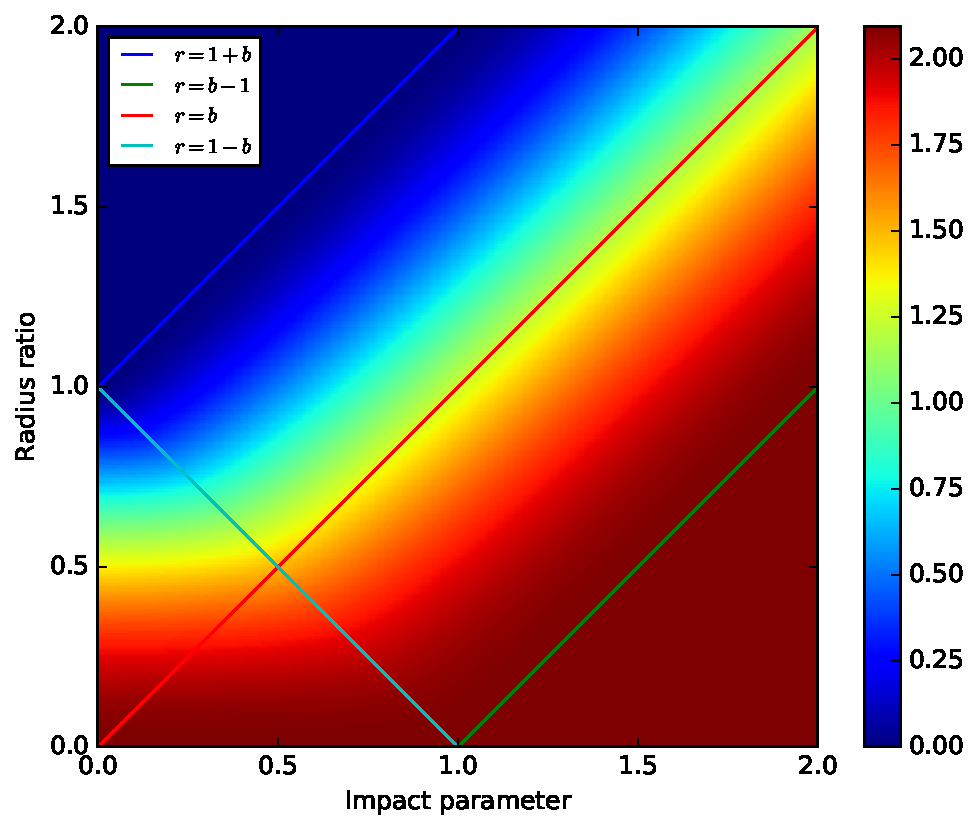
\includegraphics[width=0.85\linewidth]{figures/transit_linear.pdf}
\caption{The intensity of a linearly limb-darkened star being eclipsed, $s_2(b,r)$.
In the limit $b > r+1$, no eclipse occurs, so $s_2=1$.  For $b < r-1$, the star
is completely eclipsed and $s_2=0$.  In the limits $b=r$ and $b=1-r$, special
expressions must be used}
\end{figure}

\begin{figure}\label{s2_machine}
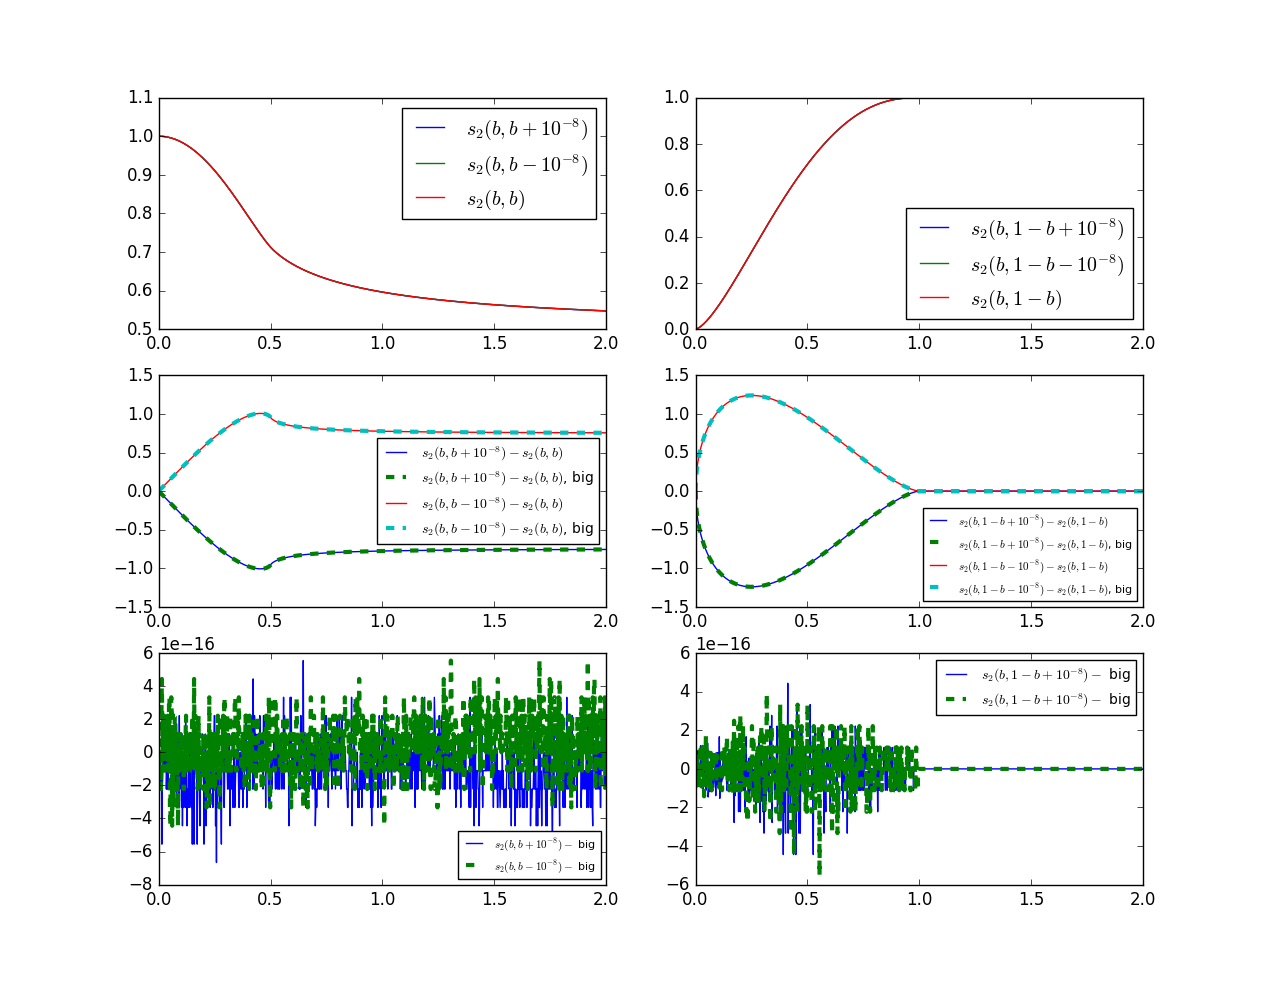
\includegraphics[width=0.85\linewidth]{figures/s2_machine.png}
\caption{The accuracy of $s_2(b,r)$ near $b=r$ (left panel) and
$b=1-r$ (right panel). The x-axese are impact parameter b,
while the y axes in the top panels show $s_2(b,r)$, with $r$
given in the legend of each panel. The middle panels plot
the difference $(s_2(b,b\pm\epsilon)-s_2(b,b))/\epsilon$
and $(s_2(b,1-b\pm\epsilon)-s_2(b,1-b))/\epsilon$. The bottom
panels show the numerical precision by the comparing double precision
computation with \texttt{BigFloat} precision (256-bit).
}
\end{figure}



%The solution for $s_2$ (Equation~\ref{eq:s2}) becomes unstable as $b \rightarrow r$ because
%the elliptic integral $\Pi$ diverges. In the vicinity of
%$b = r$ we use Equation (17.7.14) in \citet{Abramowitz1970} to express $\Pi(n, k^2)$
%in terms of Heuman's Lambda function.

%The $s_2$ term is also unstable when $r$ (and $b$) become much greater than unity, since
%in this limit $k^2 \rightarrow 0$ and $E(k^2) \rightarrow K(k^2) \rightarrow \frac{\pi}{2}.$
%Since $s_2$ depends on (among other things) a function of the difference between these two
%elliptic integrals, roundoff error in their computation leads to catastrophic cancellation
%in the result. In order to circumvent this, we re-write \eq{biglam} in terms of $E(k^2) - K(k^2)$
%and Taylor expand the expression when $r > 1$ to high order in $k^2$.

% ==============================================================================
% ------------------------------------------------------------------------------
% ------------------------------------------------------------------------------
%
\section{Quadratic Limb-Darkening}
\label{sec:quad}
% ------------------------------------------------------------------------------
% ------------------------------------------------------------------------------
% ==============================================================================

Any radially symmetric specific intensity profile can be expressed as a sum
over the $m = 0$ spherical harmonics.
%
In particular, the radial intensity profile of a quadratically
limb-darkened star,
%
\begin{align}
    \label{eq:quadraticld}
    I(\upmu) &= 1 - u_1 (1 - \upmu) - u_2 (1 - \upmu)^2
    \quad,
\end{align}
%
where $\upmu = \z = \sqrt{1 - \x^2 - \y^2}$ and $u_1$ and $u_2$ are the
limb darkening coefficients, can be written in terms of spherical harmonics
by re-writing \eq{quadraticld} as
%
\begin{align}
    I(\x, \y) = (1 - u_1 - 2u_2) + (u_1 + 2u_2) \z + u_2 \x^2 + u_2 \y^2
           \quad.
\end{align}
%
Performing the change of basis to spherical harmonics \citep{starry}, we have
%
\begin{align}
    \label{eq:qldylm}
    I(\x, \y) =
            \frac{2\sqrt{\pi}}{3} (3 - 3u_1 + 4u_2) \, Y_{0,0}
          + \frac{2\sqrt{\pi}}{\sqrt{3}} (u_1 + 2u_2) \, Y_{1,0}
          - \frac{4\sqrt{\pi}}{3\sqrt{5}} u_2 \, Y_{2,0}
      \quad.
\mathematica{limbdark}
\end{align}
%
Thus, quadratic limb darkening can be expressed exactly as the sum of the first
three $m = 0$ spherical harmonics.

\section{Radius of order impact parameter limit}

In the limit that $\vert b -r\vert \lll 1$, the edge of the occulter passes
over the center of the star.  Round-off error can cause the $s_2$ expression
to have fluctuations in the evaluation of the elliptic integral; this is
due a term that should cancel the step function...
Here we present two series expansions valid
for $\vert \epsilon \vert << 1$, where $\epsilon = b-r$, one of which is valid
for $b+r <1$ and a second for $b+r > 1$.

\subsection{$b+r <1$}

In the limit of $b+r$


\bibliography{limbdark}

\end{document}
